\subsubsection{Primary model}
\label{sec:methods_pipeline_primary_model}

The primary model consists of computing two moving average signals with
different time windows. The longer the time window, the more samples are
averaged and consequently the slower it varies with price variations. Having two
signals, one \emph{fast} and one \emph{slow} provides information of how short
and long term price movement vary one with respect to other. In particular, the
strategy takes advantage of the crossing points of both signals. When the fast
signal crosses above the slow signal, a buy event is generated. When the slow
signal crosses above the fast signal, a sell event is generated.

Note that from a daily sampled, positive and real signal as the bitcoin close
price in USD is, we obtain another two daily sampled, positive and real signals
(fast and slow). The latter two signals generate when they cross the events of
the primary model. These events are not equally spaced anymore, and the series
is categorical, its values are $\{1, -1\}$ which represent $\{buy, sell\}$
respectively. See figure \ref{fig:buy_and_sell_labels} to show these events over
the bitcoin price series.

\begin{figure}[H]
    \centering
    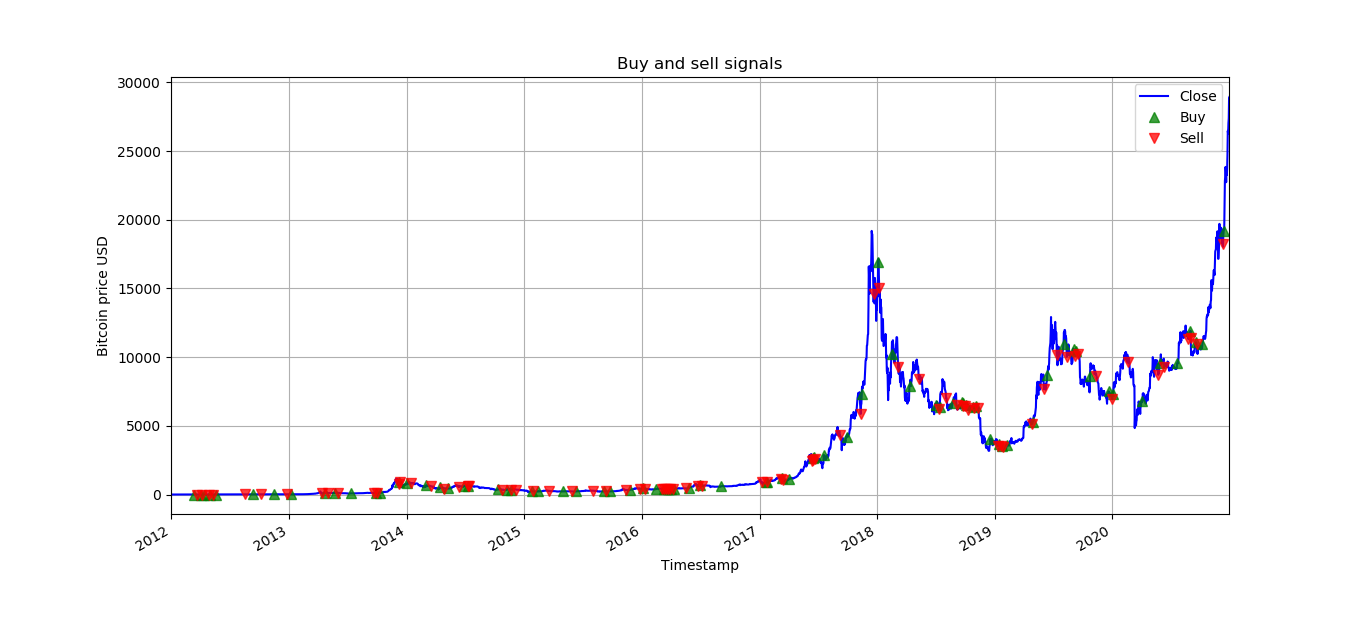
\includegraphics[width=\textwidth]{methods/images/buy_and_sell_labels.png}
    \caption{Buy and sell signals over the price series.}
    \label{fig:buy_and_sell_labels}
\end{figure}

The process of obtaining the signal with the bets is called \emph{labeling}
because it generates a series of \emph{labels} that determine a concrete action:
buy or sell the position. Next, \emph{metalabeling} process comes. It consists
in providing a probability to each \emph{label} which will be used to size the
bet. To assess whether the \emph{label} is correct or not, the triple barrier
method is used:

\begin{enumerate}
  \item Define a profit taking and stop loss rate for which a buy and sell
        signals will be considered valid. For a given price and time, a new
        greater value and lesser value are defined based on both rates before.
  \item Define a time constant $h$ (expressed as a positive and integer multiple
        of the sampling rate, i.e. number of days) that determines for each
        label, a new time stamp ahead.
  \item Determine whether the price signal hits the greater price or the lesser
        price before reaching the time stamp ahead of $h$ periods from the
        label's event. When:
  \begin{itemize}
    \item A $1$-valued label gets a cross with the greater price barrier, the
          metalabel is $1$ to indicate a positive label.
    \item A $-1$-valued label gets a cross with the lesser price barrier, the
          metalabel is $1$ to indicate a positive label.
    \item A $1$-valued label gets a cross with the lesser price barrier, the
          metalabel is $0$ to indicate a positive label.
    \item A $-1$-valued label gets a cross with the greater price barrier, the
          metalabel is $0$ to indicate a positive label.
    \item When both $1$ and $-1$ valued labels do not get a corresponding cross 
          with any of the price barriers, the return sign between the price at
          $h$ sample periods ahead of label's time stamp and the label's price
          is used. If the sign of the return and the label match, the metalabel
          is $1$, otherwise it is $0$.
  \end{itemize}
\end{enumerate}

Labels and metalabels are fundamental series to build the secondary model. The
secondary model is a classifier that is trained with metalabels. The predicted
probability will help to size the bet on each label. In mathematical terms:
$Metalabels = f_{(Labels, ...)}$ where $f$ represents the secondary model.